\documentclass[11pt, oneside]{article}   	% use "amsart" instead of "article" for AMSLaTeX format
\usepackage{geometry}                		% See geometry.pdf to learn the layout options. There are lots.
\geometry{letterpaper}                   		% ... or a4paper or a5paper or ... 
%\geometry{landscape}                		% Activate for for rotated page geometry
%\usepackage[parfill]{parskip}    		% Activate to begin paragraphs with an empty line rather than an indent
\usepackage{graphicx}				% Use pdf, png, jpg, or eps with pdflatex; use eps in DVI mode
								% TeX will automatically convert eps --> pdf in pdflatex		
\usepackage{amssymb}
\graphicspath{{/Users/telliott_admin/Dropbox/Tex/png/}}

\title{Volume of rotated ellipse}
%\author{The Author}
\date{}							% Activate to display a given date or no date

\begin{document}
\maketitle
%\section{}
%\subsection{}

We want to calculate the volume generated by rotation of an ellipse (centered at the origin) about the x-axis.

\begin{center}
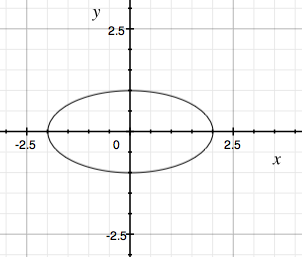
\includegraphics [scale=0.5] {ellipse.png}
\end{center}

The basic idea is that the cross-section of each little slice in the direction we are integrating is a circle with radius equal to f(x).
\[
y = f(x)
\]
The area of each slice is a function of x, given by
\[
A = \pi \ y^2
\]
We add up all those little slices by doing this integral
\[
V = \pi \int y^2 \ dx
\]
For the general ellipse we have the equation
\[
\frac{ x^2 }{ a^2 } + \frac{ y^2 }{ b^2 } = 1
\]
\[
y^2 =  b^2 (1 - \frac{ x^2 }{ a^2 })
\]
So the integral is
\[
V = \pi \int y^2 dx = \pi \int b^2 (1 - \frac{ x^2 }{ a^2 }) \ dx
\]
which is just
\[
V = \pi b^2 \ ( x - \frac{ x^3 }{ 3a^2 } )
\]
evaluated between x = -a and x = a
\[
V = \pi  b^2 [ (a - \frac{a}{3}) - (-a - \frac{-a}{3}  ) ] =  \frac{4}{3} \pi b^2 a
\]

We get a squared contribution for the b component, which describes the "stretching" of the ellipse in the direction of the axis of rotation.  Rotation around the y-axis would give a formula containing a squared, and a bigger solid by a factor of a/b.

\end{document}  